% 候选插图片段：选择后再加入正文，不一次性全部引用。
% 已存在的 graphicspath 若只含 figures/，文件名前保留 p34_candidates/。

\begin{figure}[htbp]
\centering
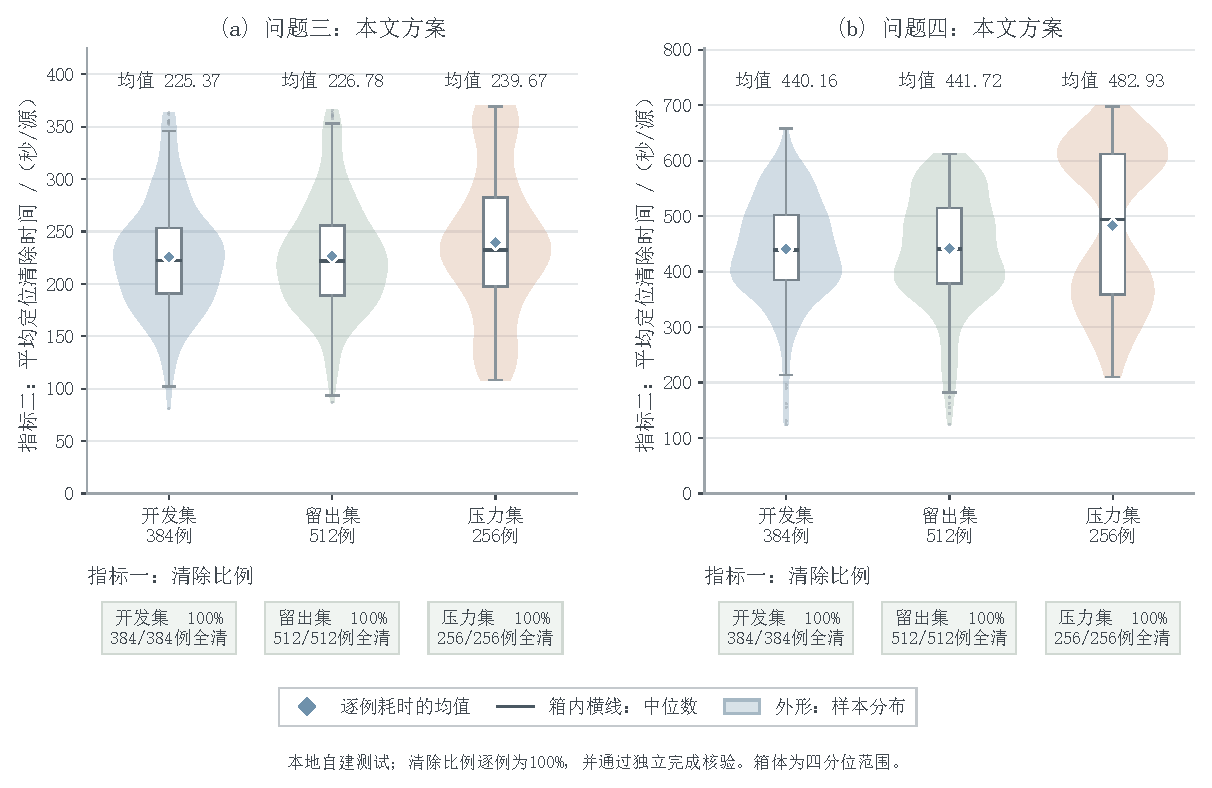
\includegraphics[width=0.98\linewidth]{p34_candidates/01_local_two_metrics.pdf}
\caption{本地测试的两项实际指标（本地结果或机制示意，详见候选图注）}
\label{fig:p34-candidate-01}
\end{figure}

\begin{figure}[htbp]
\centering
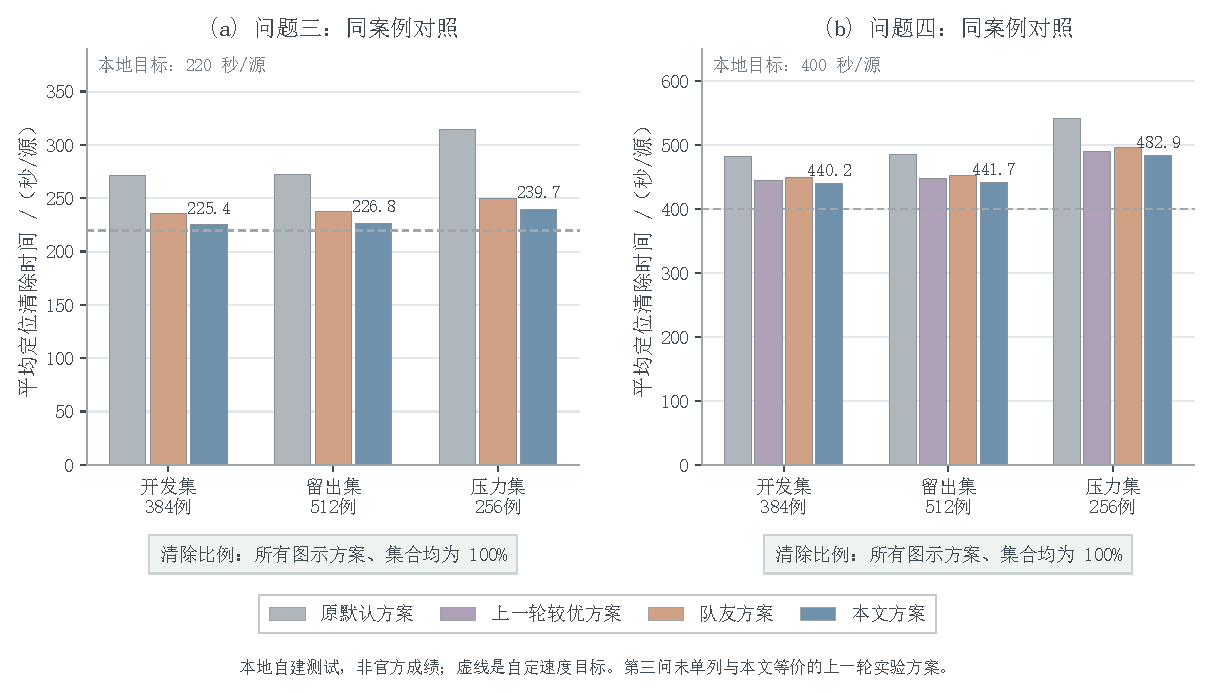
\includegraphics[width=0.98\linewidth]{p34_candidates/02_metrics_comparison_bars.pdf}
\caption{两项指标的方案对照：柔和分组柱图（本地结果或机制示意，详见候选图注）}
\label{fig:p34-candidate-02}
\end{figure}

\begin{figure}[htbp]
\centering
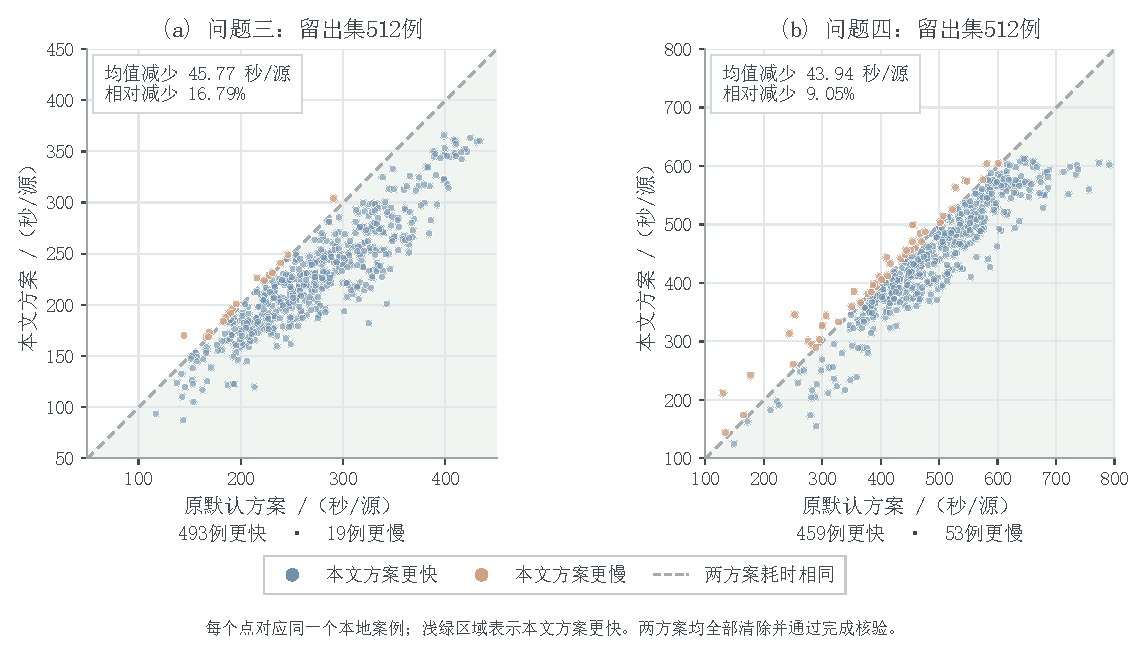
\includegraphics[width=0.98\linewidth]{p34_candidates/03_paired_case_comparison.pdf}
\caption{留出案例的逐例速度比较（本地结果或机制示意，详见候选图注）}
\label{fig:p34-candidate-03}
\end{figure}

\begin{figure}[htbp]
\centering
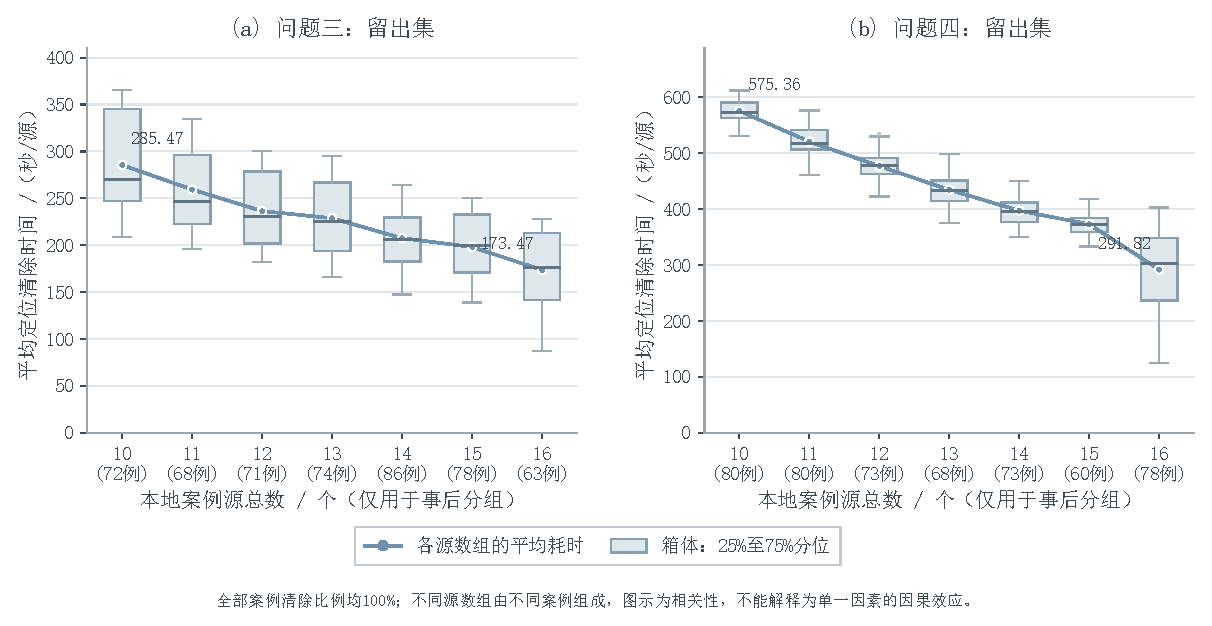
\includegraphics[width=0.98\linewidth]{p34_candidates/04_time_by_source_count.pdf}
\caption{源数量与每源耗时的关系（本地结果或机制示意，详见候选图注）}
\label{fig:p34-candidate-04}
\end{figure}

\begin{figure}[htbp]
\centering
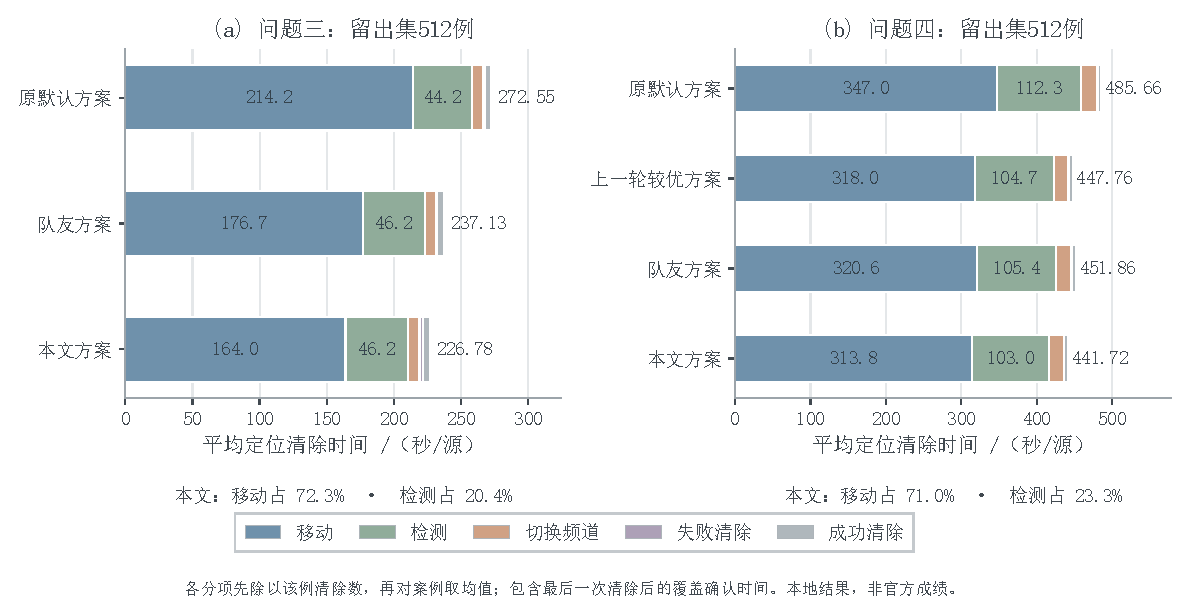
\includegraphics[width=0.98\linewidth]{p34_candidates/05_time_cost_breakdown.pdf}
\caption{平均定位清除时间的构成（本地结果或机制示意，详见候选图注）}
\label{fig:p34-candidate-05}
\end{figure}

\begin{figure}[htbp]
\centering
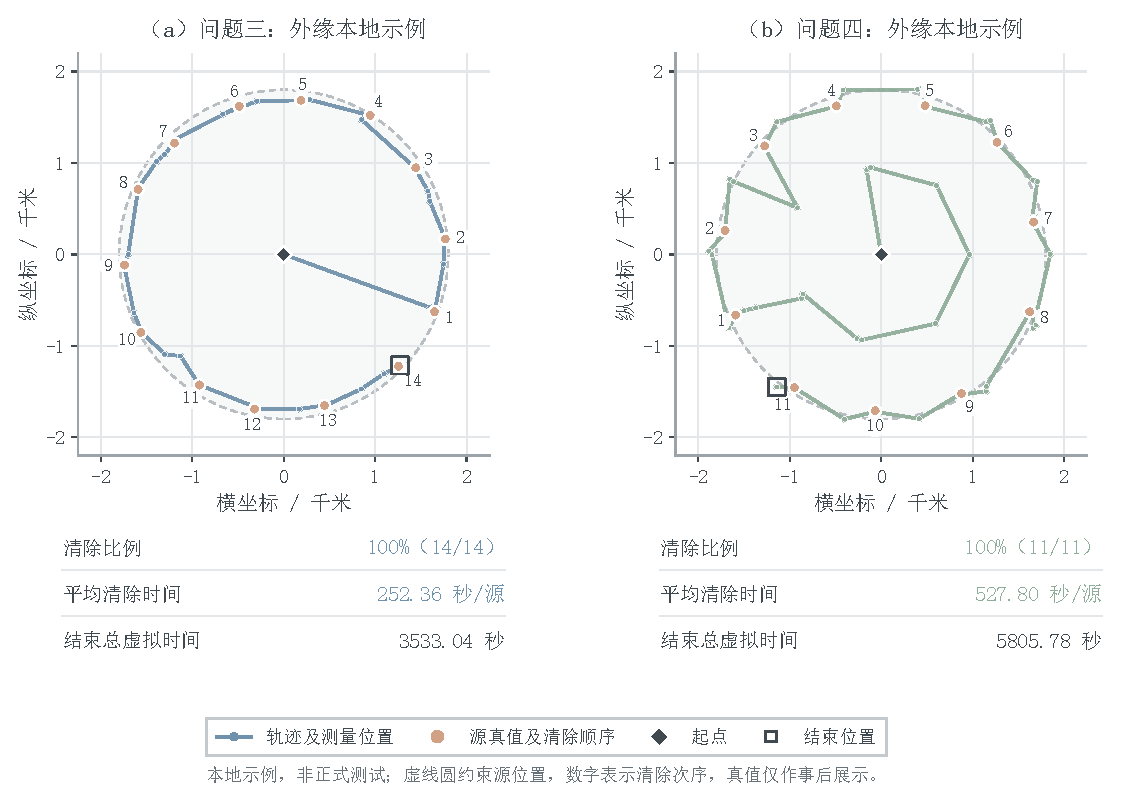
\includegraphics[width=0.98\linewidth]{p34_candidates/06_case_routes.pdf}
\caption{本地外缘示例的搜索轨迹与两项指标（本地结果或机制示意，详见候选图注）}
\label{fig:p34-candidate-06}
\end{figure}

\begin{figure}[htbp]
\centering
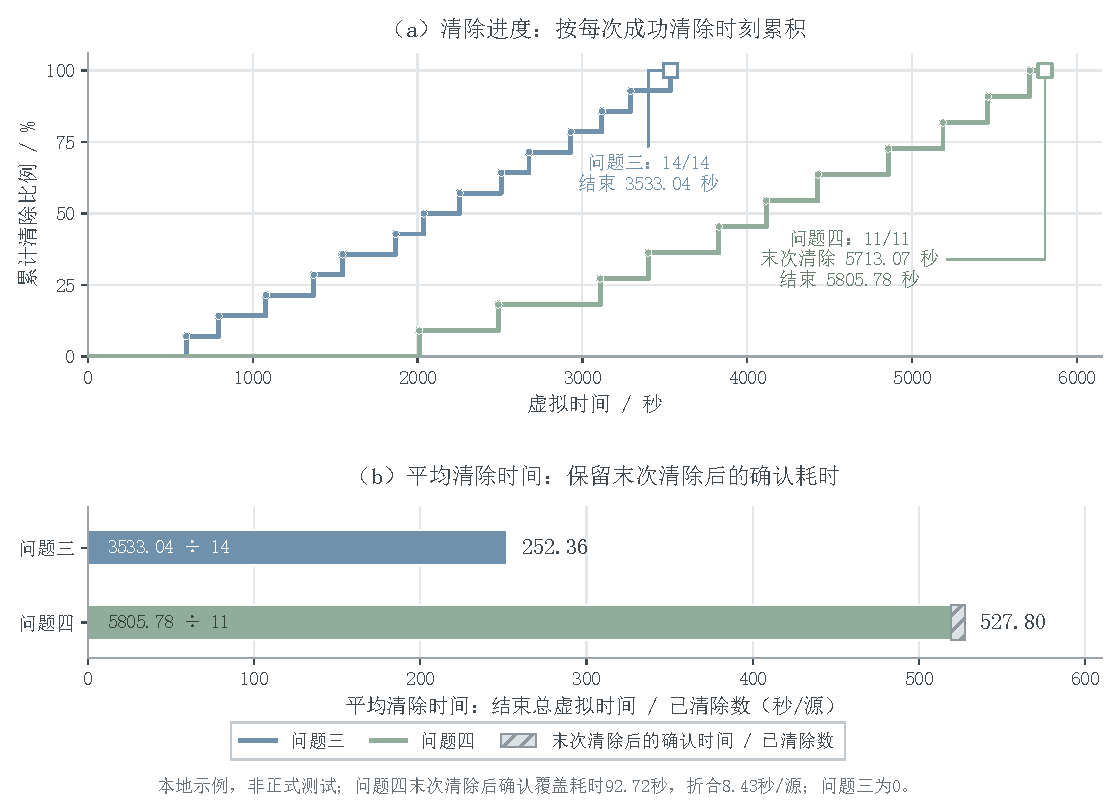
\includegraphics[width=0.98\linewidth]{p34_candidates/07_case_progress.pdf}
\caption{本地外缘示例的清除进度与平均清除时间（本地结果或机制示意，详见候选图注）}
\label{fig:p34-candidate-07}
\end{figure}

\begin{figure}[htbp]
\centering
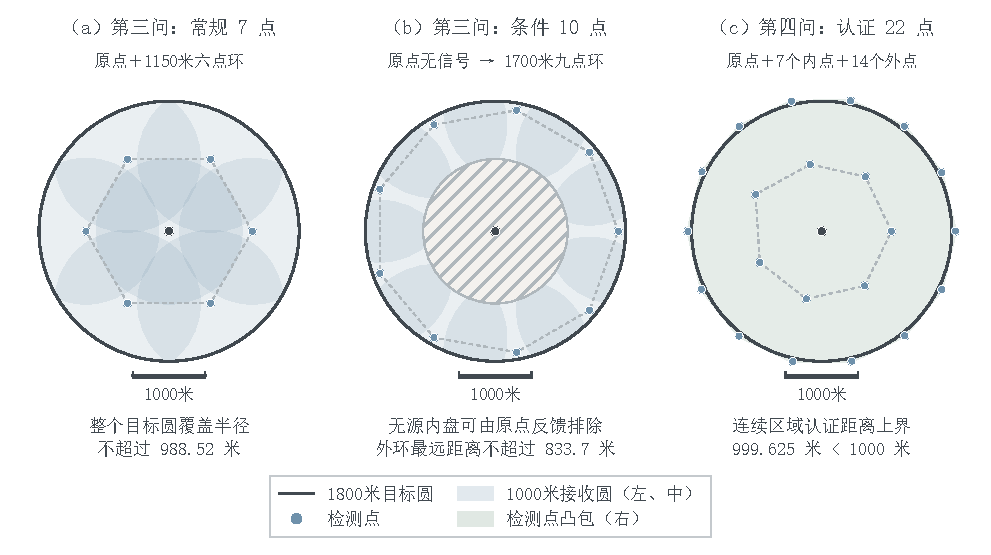
\includegraphics[width=0.98\linewidth]{p34_candidates/08_coverage_layouts.pdf}
\caption{第三、四问的条件覆盖与认证布局（本地结果或机制示意，详见候选图注）}
\label{fig:p34-candidate-08}
\end{figure}

\begin{figure}[htbp]
\centering
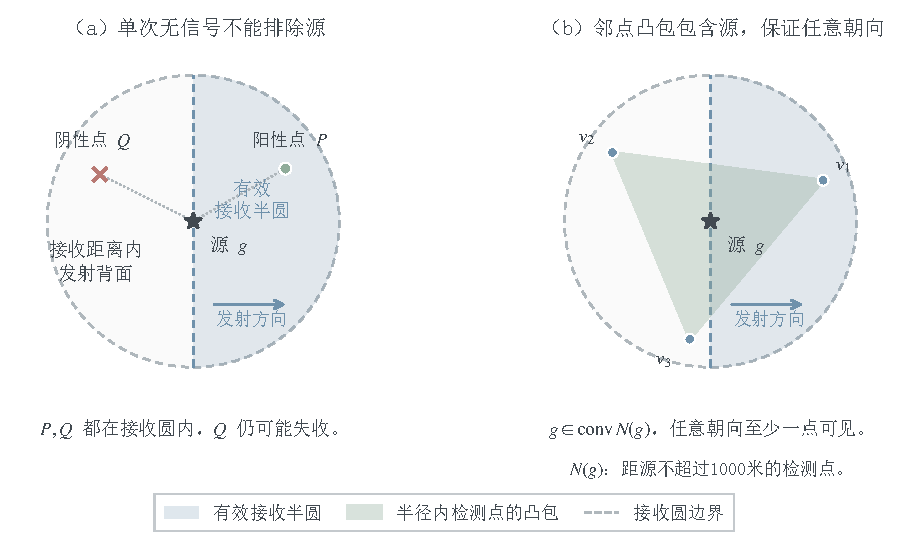
\includegraphics[width=0.98\linewidth]{p34_candidates/09_directional_visibility.pdf}
\caption{定向接收的阴性歧义与凸包覆盖条件（本地结果或机制示意，详见候选图注）}
\label{fig:p34-candidate-09}
\end{figure}

\begin{figure}[htbp]
\centering
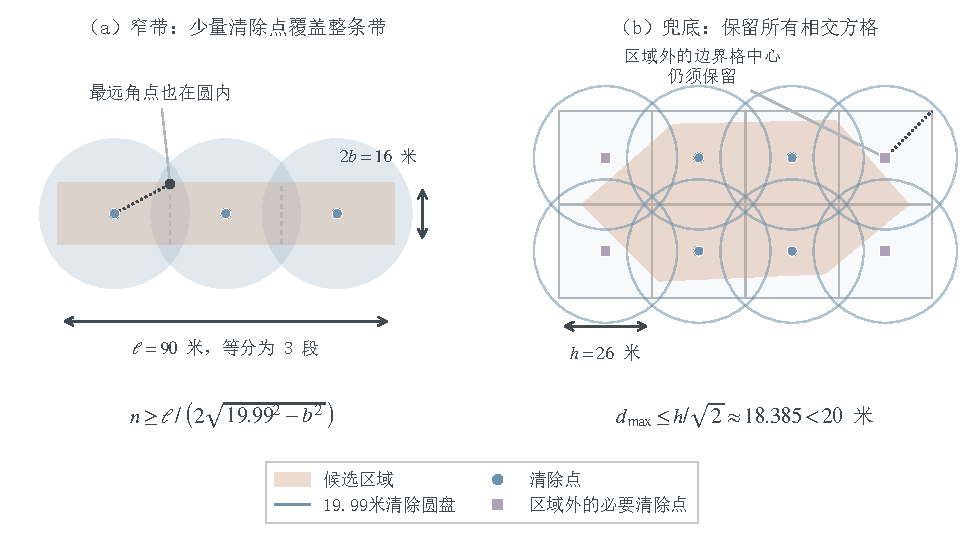
\includegraphics[width=0.98\linewidth]{p34_candidates/10_optical_cover.pdf}
\caption{窄带光学清除与完整网格兜底（本地结果或机制示意，详见候选图注）}
\label{fig:p34-candidate-10}
\end{figure}
